%% The first command in your LaTeX source must be the \documentclass command.
%%
%% Options:
%% twocolumn : Two column layout.
%% hf: enable header and footer.
\documentclass[
% twocolumn,
% hf,
]{ceurart}

%%
%% One can fix some overfulls
% \sloppy

%%
%% Minted listings support
%% Need pygment <http://pygments.org/> <http://pypi.python.org/pypi/Pygments>
\usepackage{minted}
\usepackage{multicol}
%% auto break lines
\setminted{breaklines=true}
\usepackage{doi}
\def\doitext{DOI:}
% \newcommand{\doi}[1]{DOI:#1}
\graphicspath{{pics/}}

%%
%% end of the preamble, start of the body of the document source.
\begin{document}

%%
%% Rights management information.
%% CC-BY is default license.
\copyrightyear{2021}
\copyrightclause{Copyright for this paper by its authors.
  Use permitted under Creative Commons License Attribution 4.0
  International (CC BY 4.0).}

%%
%% This command is for the conference information
\conference{ITAMS'2021: Information Technologies: Algorithms, Models, Systems. September 17${}^{th}$, 2021, Irkutsk, Russia}

%%
%% The "title" command
\title{Web-GIS viewer for active faults data represented as a knowledge graph}

%%
%% The "author" command and its associated commands are used to define
%% the authors and their affiliations.
\author[1,3,4]{Evgeny A. Cherkashin}[%
orcid=0000-0003-2428-2471,
email=eugeneai@icc.ru,
url=https://github.org/eugeneai,
]
\address[1]{Matrosov Institute for System Dynamics and Control Theory of Siberian Branch of Russian Academy of Sciences, 134 Lermontov St, Irkutsk, 664033, Russian Federation}

\author[2]{Oksana V. Lunina}[%
orcid=0000-0001-7743-8877,
email=lounina@crust.irk.ru,
url=http://www.crust.irk.ru/member_88.html,
]

\address[2]{Institute of the Earth’s Crust of Siberian Branch of Russian Academy of Sciences, 128 Lermontov St, Irkutsk, 664033, Russian Federation}

\author[3]{Leonid O. Demyanov}

\address[3]{Institute for Mathematics and Informational Technologies, Irkutsk State University, 20~Gagarina Bulv, Irkutsk, 664003, Russian Federation}

\author[4]{Alexander V. Tsygankov}

\address[4]{Institute for Information Technologies and Data Analysis, National Research Irkutsk State Technical University, 83~Lermontov St, Irkutsk, 664074, Russian Federation}

%%
%% The abstract is a short summary of the work to be presented in the
%% article.
\begin{abstract}
  A problem of flexible geographical data representation and Web-based visualization is considered.  The data stored in a knowledge graph as ontologies (vocabularies) in accordance to W3C standards.  For viewing data, a web geographical information system (GIS) application is realized, which renders map interpreting SPARQL queries to Sematic Web server storing the knowledge graph.  The technologies used for designing are based on contemporary Web 3.0, allowing one to implement Linked Open Data compliance for GIS information publishing and integration.
\end{abstract}

%%
%% Keywords. The author(s) should pick words that accurately describe
%% the work being presented. Separate the keywords with commas.
\begin{keywords}
  geographical information system \sep
  knowledge graph \sep
  semantic web \sep
  storing flexible data \sep
  one-page web application
\end{keywords}

%%
%% This command processes the author and affiliation and title
%% information and builds the first part of the formatted document.
\maketitle

\section{Introduction}

Contemporary Web technologies development is aimed at more tight data integration: standardization of data publishing formats, formal data and metadata representation, unifying interpretation contexts, referring to external entities.  Geospatially related objects are frequently published in the requirements as well.

Geospatial data are of primary interest of people as many human activities are attached to object located on the Earth's surface.  There are a lot of on-line services helping users to navigate, figure out the places corresponding the required conditions (shopping centers, parking places, \emph{etc.}), observation of territories to familiarize themselves.  The objects of interest as any data objects are described with attributes of various kinds, like working hours of firms, their home site URLs, nearby bus stations.  At present, these software products trend to allow integration with their data via open formats and publishing principles, \emph{e.g.}, Linked Open Data.

In this investigation, the fault data are chosen as subject for representation and publishing.  Geological field investigations and event observations, \emph{e.g.}, earthquakes, accumulate data, which are analyzed, resulting in setting new attributes to a fault or their refinement.  According to the techniques of geological research, additional information are associated with attributes, clarifying their values.  Such clarification comprises precision characteristics, measurement conditions, reliability assessment, and paper references, where fault data were published.

GIS\footnote{Abbreviation of Geographical Information System} represents spatial data in semantic defined layers.  For each object of a layer, one can associate a set of attribute values of auxiliary data.  The set of the attributes are the same for each object of the layer regardless of whether the attribute value is defined for an object or not.  Empty values are represented as ``\texttt{null}''s.  In the case of geological exploration, when a lot of attributes are undefined, this approach leads to sparse filled tables.  This, in turn, requires data modification and analysis algorithms to utilize additional data checking stages when using standard relation operations (SELECT, UPDATE, DELETE).

Another question is attribute names definition expressing semantics of metadata.  For example, to define a precision of a value one could construct an attribute name with ``\texttt{\_prec}'' suffix, where name is its value attribute identifier.  Other types of metadata add more suffixes, as well as relations between suffixes and values are not defined anywhere in the database.  The formal definition is to be defined in a documentation or processing algorithms, thus, either informally defined or obfuscated, and practically not alienated.  Adding new attributes requires the user to devise new synthetic names.

Web publication applications, as information systems, are to implement filtering functions, differentiating the value attributes and their metadata.  Screen widgets label names either defined in application or figured out from the attribute names.  Lack of ontological (vocabulary) formal domain definition forces developer to spend more efforts for user interface implementation.

Since 2001 Semantic Web technologies have evolved in a substantial set of instruments for data storing, publishing, and software integration, allowing system designers and programmers, among standard means, to pass data between systems via published documents and application user interfaces, \emph{i.e.}, extending their set of functions.  Vocabularies and data instances are stored in graph databases, which provide SPARQL and other endpoints on top of HTTP protocols, enabling similar services as relational database servers for data access and modification.  The generalized problem statements and approaches to their solutions in the field of Semantic Web are the reasons of its constant development.

Knowledge graphs (KG) \cite{hogan} are techniques of Semantic Web usage aimed at representation of data in a general flexible way allowing so-called ``natural'' evolving of domain image, including representation of incomplete knowledge.  This evolution corresponds to a scientific research process, where data is accumulated and analyzed.  KG enables both providing in addition distributed storage, federated query based access and modification, means for metadata definition, and formalized verification of its content.

The aim of this research and development is to represent existing tabular and spatial data from \cite{lunina,afs} as a knowledge graph with implementing a viewer, assessing ``working efficiency'' of a programmer and ``usability'' of KG services.  State further development perspectives, ranging them by priorities.

\section{Data conversion}

The original database structure is shown in Figure~\ref{fig:db-struct}.  This structure contains  field ``\texttt{ID}'' defining fault identifier, the fault name as a geographical entity, various characteristics with corresponding clarifications, seismic activity, name of compiler researcher and date of refinement.  Data is stored in \texttt{DBF} format, the record number relates the database record with spatial object of fault layer.  Field names in \texttt{DBF} file cannot be longer than ten characters, must be in capitalized, number of fields cannot be more than 255.
\begin{figure}
  \centering
  \footnotesize
    \begin{multicols}{2}
\begin{verbatim}
!table
!version 300
!charset WindowsCyrillic

Definition Table
  Type NATIVE Charset "WindowsCyrillic"
  Fields 72
    ID Char (15) Index 1 ;
    Name Char (40) Index 2 ;
    Location Char (250) Index 3 ;
    Strike Char (10) Index 4 ;
    Strike_Q Char (2) ;
    Dip_azimuth Char (10) Index 5 ;
    Dip_azimuth_Q Char (2) ;
    Dip_angle Char (10) Index 6 ;
    Dip_angle_Q Char (2) ;
    Length_km Char (10) Index 7 ;
    Length_Q Char (2) ;
    Depth_km Char (10) Index 8 ;
    Depth_Q Char (2) ;
    Width_damage_zone_km Char (10) Index 9 ;
    Width_damage_zone_Q Char (2) ;
    Slip_sense Char (30) Index 10 ;
    Slip_sense_Q Char (2) ;
    Slip_sense_Index Decimal (2, 0) ;
    Total_Cenozoic_lateral_slip_m Char (20) ;
    Total_Cenozoic_lateral_slip_Q Char (2) ;
    Total_Cenozoic_vertical_slip_m Char (20) ;
    Total_Cenozoic_vertical_slip_Q Char (2) ;
    . . . . . . . . . . . . . . . . . . . .
    Potential_Ms_max Float ;
    Potential_Ms_max_Q Char (2) ;
    Potential_Mw_max Float ;
    Potential_Mw_max_Q Char (2) ;
    Elapsed_time_years Char (10) ;
    Elapsed_time_Q Char (2) ;
    Associated_CSS Char (25) ;
    Associated_IGGSS Char (50) ;
    Seismic_activity_of_fault Char (3) ;
    Compiler Char (50) ;
    Date Char (10) ;
\end{verbatim}
  \end{multicols}
  \caption{Part of the structure of the original database}
  \label{fig:db-struct}
\end{figure}

  Identifiers of the attributes with common prefixes define one value with a clarification, \emph{e.g.}, ``\texttt{Depth}'' and ``\texttt{Length}'' of a fault are measured in kilometers, their values are clarified with ``quality'' attribute having suffix ``\texttt{\_Q}'' at the end.

  Table content slice of the fault database is shown in Figure~\ref{fig:db-slice}.  It is sparse filled: many attributes are \texttt{null}s.  The field ``\texttt{Geomorphol\ldots}'' and some others is filled with values of predefined sets.  The consistency are controlled algorithmically with QGIS extension modules.  This flat structure and representation format are intended to be easily accessed and realized with standard relational database tools, but general violations of standard normal forms forces the developer to implement additional subroutines controlling a record content (semantics) in addition to the UPDATE DML\footnote{Abbreviation of Data Manipulation Language.} command.

  \begin{figure}
    \centering
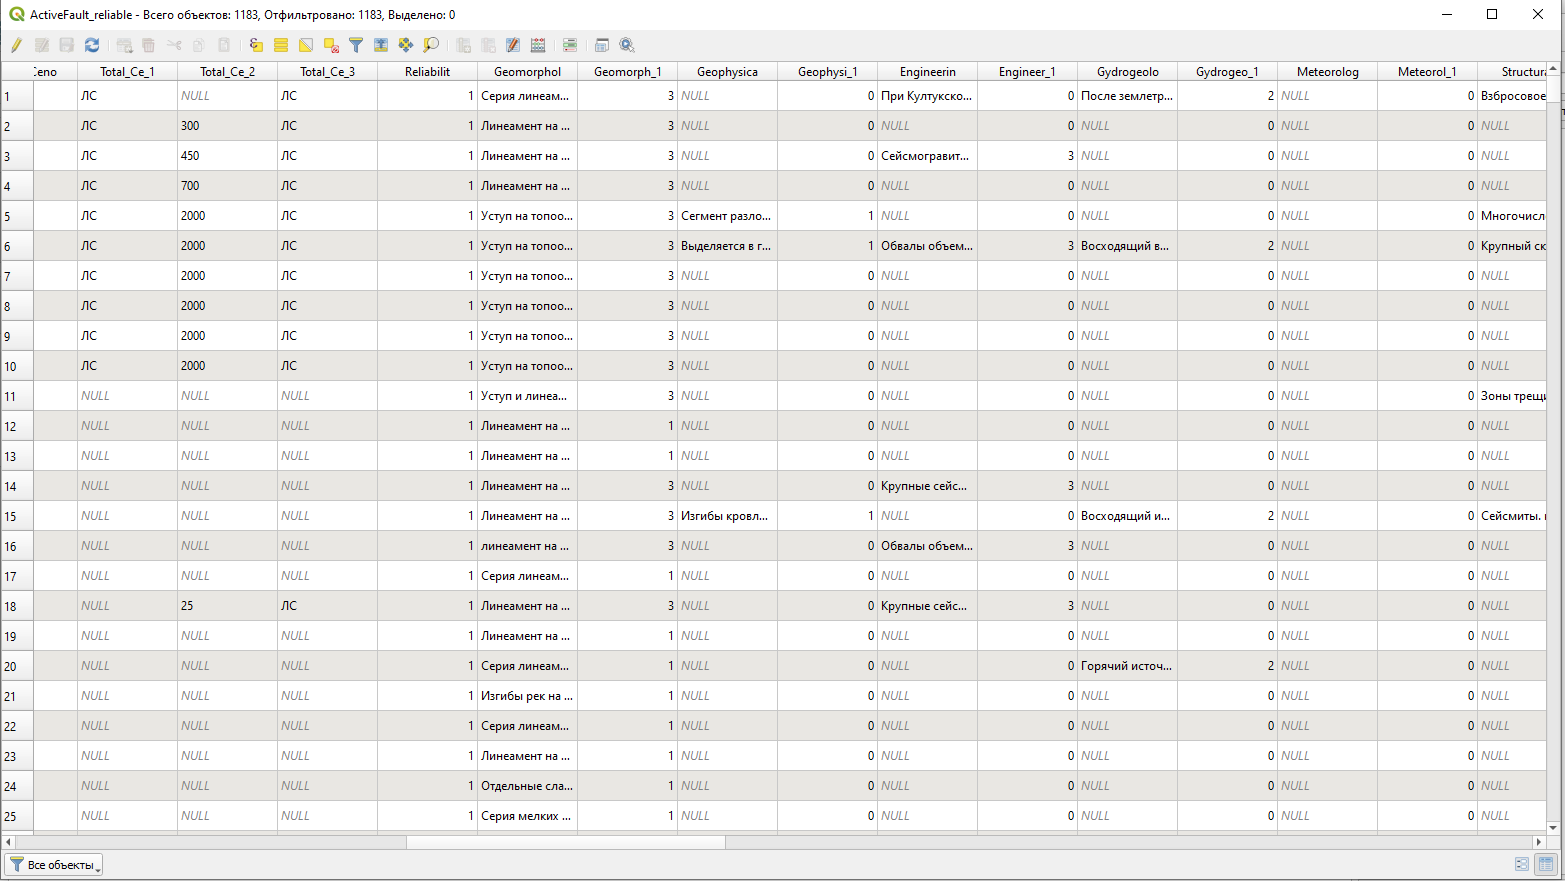
\includegraphics[width=\linewidth]{faults-leaflet-db-content.png}
    \caption{A table content slice}
    \label{fig:db-slice}
  \end{figure}

Conversion started with defining T-Box\footnote{Abbreviation of Terminological Box, a set of basis domain terms and their relationships.} comprising the class of fault and its subclasses.  Subclasses correspond to various kinds of faults, \emph{e.g.}, normal, reverse, strike-slip, oblique.  As a differentiating property, ``\texttt{Slip\_sense}'' attribute used.  All the fault records when converted and assigned a class formed A-Box\footnote{Denotation of Instance Box, a set of the instances.}, a database of faults.  Non-\texttt{null} attributes of faults were converted into a literal relation, except those, which values were restricted to a finite set.  These attribute values presented as references to a descriptive constant added to T-Box.  These conversions were implemented as Python program loading \texttt{DBF}-files and generation \texttt{OWL2} \texttt{XML} ones.  After the conversion, the obtained \texttt{OWL}s of T-Box and A-Box were visually checked with Protégé, saved into Turtle (\texttt{ttl}) format.

The results of conversions were manually loaded into GraphDB and Jena KG servers.  For each part (T- and A-Box) a global namespace (\texttt{aft}, \texttt{af}) were allocated: \url{http://irnok.net/ontologies/ActiveFaultTerms\#} and \href{http://irnok.net/ontologies/ActiveFault\#}{\ldots/ActiveFault\#}.  In the software, for each KG one must set up an individual endpoint providing access.  GraphDB user interface were used to check the correctness of class-instance relations with executing SPARQL-queries.  The peculiarity of GraphDB usage is the necessity to ``activate'' each KG endpoint via user interface after loading their KG contents.  After conversion and set up of the endpoint they will be available at port 7200, URL will be formed out of server address and endpoint name.  An example of a converted item is shown here

\begin{multicols}{2}\tiny
  \begin{verbatim}
###  http://irnok.net/ontologies/ActiveFaults#RUAF_996
af:RUAF_996 rdf:type owl:NamedIndividual ,
      aft:Fault ,         # Classification
      aft:NormalSlCB ,
      aft:PlioceneFault ;
   aft:ID "RUAF_996"^^xsd:string ;
   aft:Activity_degree aft:Light ;
   aft:Averaged_slip_rate [ aft:value "0.0"^^xsd:float ;
       aft:unit aft:Millimeter ] ;
   aft:Compiler "Lunina O.V."^^xsd:string ;
   aft:Date "29.05.2011"^^xsd:string ;
   aft:Dip_azimuth [ aft:value "310"^^xsd:string ;
       aft:quality aft:LC ] ;
   aft:Engineering_geological_grade [ aft:value "0"^^xsd:int ] ;
   aft:Geomorphological_features [
       aft:value "Topographic ledge: 1 point"^^xsd:string ;
       aft:grade "1"^^xsd:int ] ;
   aft:Geophysical_grade [ aft:value "0"^^xsd:int ] ;
   aft:Gydrogeological_grade [ aft:value "0"^^xsd:int ] ;
   aft:Last_activation_age [ aft:value aft:Pliocene ;
       aft:ageindex "4.0"^^xsd:float ] ;
   aft:Lateral_max_slip_per_event [ aft:value "0.0"^^xsd:float;
       aft:unit aft:Meter ] ;
   aft:Length [ aft:value "12.09"^^xsd:string ;
       aft:quality aft:LC ;
       aft:unit aft:Kilometer ] ;
   aft:Location "At the edge of Barguzin depression and \
       Ikatsky ridge"^^xsd:string ;
   aft:Meteorological_grade [ aft:value "0"^^xsd:int ] ;
   aft:Paleoseismological_grade [ aft:value "0"^^xsd:int ] ;
   aft:Potential_Ms_max [ aft:value "0.0"^^xsd:float ] ;
   aft:Potential_Mw_max [ aft:value "0.0"^^xsd:float ] ;
   aft:Reliability_class [ aft:value "1.0"^^xsd:float ] ;
   aft:Seismic_activity_of_fault [ aft:value "false"^^xsd:boolean ] ;
   aft:Seismological_grade [ aft:value "0"^^xsd:int ] ;
   aft:Slip_rate_grade [ aft:value "0"^^xsd:int ] ;
   aft:Slip_sense [ aft:value aft:Discard ;
       aft:index "1.0"^^xsd:float ;
       aft:quality aft:LC ] ;
   aft:Strike [ aft:value "40"^^xsd:string ;
       aft:quality aft:LC ] ;
   aft:Structural_geological_grade [ aft: value "0"^^xsd:int ] ;
   aft:Total_activity_grade [ aft:value "1.0"^^xsd:float ] ;
   aft:Total_max_slip_per_event [aft:value "0.0"^^xsd:float ;
       aft:unit aft:Meter ] ;
   aft:Vertical_max_slip_per_event [ aft:value "0.0"^^xsd:float ;
       aft:unit aft:Meter ] ;
   aft:Width_damage_zone [ aft:value "1.21"^^xsd:string ;
       aft:quality aft:AC ;
       aft:unit aft:Kilometer ] .
\end{verbatim}
\end{multicols}

\section{Viewer implementation}

Our viewer is a Web-2.0 application composed out of React components.  The application maintains its state with Redux. Properly used Redux allows one to control viewer widgets content and structures solely by defining state change functions.

Rendering maps is based on React wrapper of \texttt{leaflet.js} library.  The library allows one to draw interactive graphics objects (polygons) on a topological basis.  Leaflet supports various sources, such as \href{https://openstreetmap.org/}{openstrrtmpa.org}, which is default one.  Fault shapes were converted from \texttt{KML} format to leaflet interpretable \texttt{JSON} and are being loaded by application on demand from web server.

By default, viewer shows all faults from KG, the result of a SPARQL query requesting all objects of a class \texttt{aft:Fault}\footnote{\url{http://irnok.net/ontologies/ActiveFaultTerms\#Fault}}, \emph{i.e.} all the instances\footnote{All faults are instances of \texttt{aft:Fault}}.  There is a form in the user interface for setting filtering conditions.  They change the default SPARQL query, adding restrictions.  For the debugging and developing, one version of the viewer contains a form for free-form SPARQL query definition, which execution results also showed as a fault map.

Viewing fault attributes is implemented as a form document improved with \texttt{RDFa} markup.  This markup originates from results of SPARQL query selecting all the predicate relation for the chosen fault.
%
% \subsection{Examples of the usage}
%
In Figure~\ref{fig:ex}, viewer window is shown.  As a subject of interest, Irkut-Ushakovsky fault being extended through Irkutsk city is chosen.

\begin{figure}
  \centering
  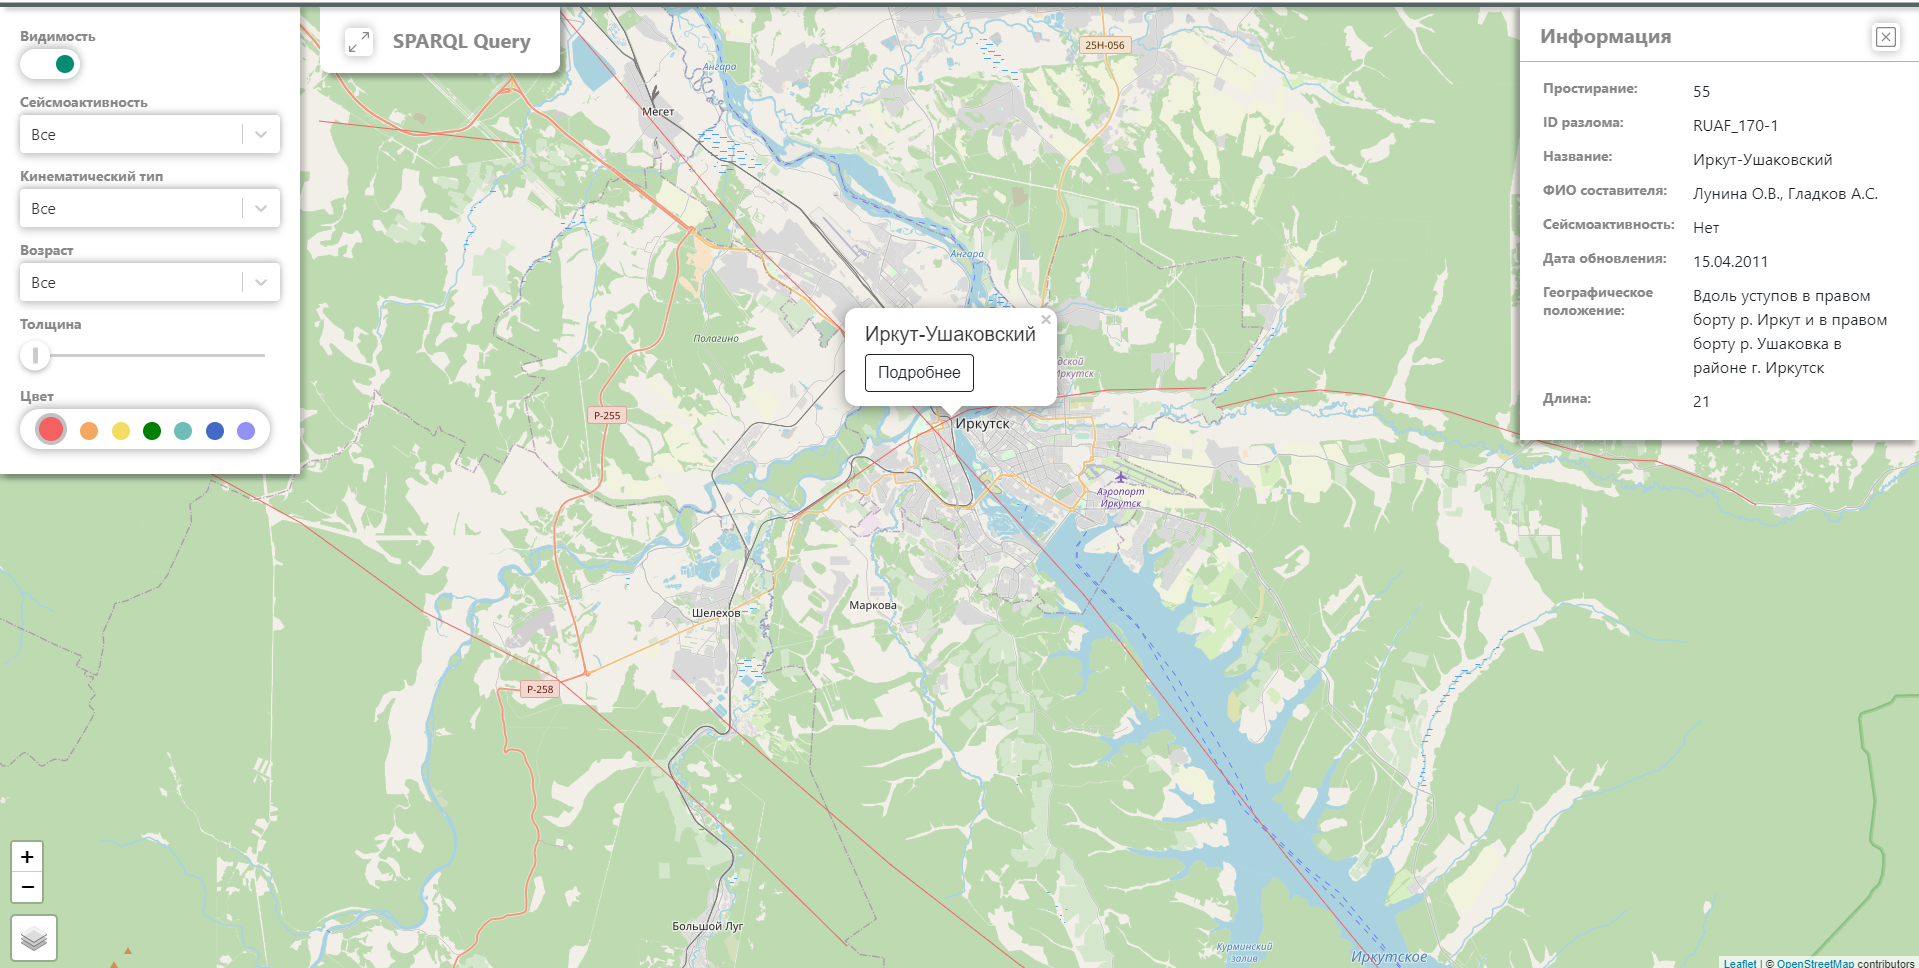
\includegraphics[width=\linewidth]{faults-leaflet-doc.png}
  \caption{Viewer window showing description of a fault}
  \label{fig:ex}
\end{figure}


\section{Related Works}

  The project\footnote{Claus Stadler, Jens Lehmann, Konrad Höffner, Sören Auer. LinkedGeoData:
A core for a web of spatial open data. Semantic Web 3 (2012) 333–354. \doi{10.3233/SW-2011-0052}} was to represent OpenSteetMap (OSM) data as a KG,
  \begin{itemize}
  \item Resembles the DBPedia project formalizing Wikipedia data but over the OSM database
  \item Converts SM data into RDF adhering LOD
  \item Designed an ontology for object georeferencing (nodes)
  \item Related the object to DBpedia, GeoNames, icon sets
  \item Developed a taxonomy of the objects on a various levels (Road~\to~Way (list of nodes)) % and Fig 3 of the LGD paper.
  \item Stated the relations between nodes and ways defining complex objects
  \item Implemented REST and SPARQL (does not work now) endpoints for actual data
  \item Had a live updates services from OSM change sets.
  \end{itemize}


    GeolLink KG\footnote{Michelle Cheatham, Adila Krisnadhi, Reihaneh Amini, Pascal Hitzler, \emph{et al} (2018) The GeoLink knowledge graph, Big Earth Data, 2:2, 131-143, \doi{10.1080/20964471.2018.1469291}}
  \begin{itemize}
  \item Includes diverse information as port calls made by oceanographic cruises, physical sample metadata, research project funding and staffing, and authorship of technical reports
  \item Implements LOD (4 of 5 stars) and federated SPARQL integration
  \item Contains 45 millions RDF triples with ontologies and geo-visualization tools
  \item Describes interlinked \textbf{R2R}, expeditions, \textbf{BCO-DMO}, oceanography, \textbf{IODP}, ocean floor microbiome, \textbf{MBLWHOI}, marine life papers, \textbf{SESAR}, rock samples, \textbf{DataONE}, metadata of external research,  \textbf{AGU-NSF}, projects \& conferences, \textbf{NGDB}, sediment geochemy, \textbf{USAP}, Antarctica ice.
  \end{itemize}
  In the project, an update procedure (harvesting) is implemented to ensure the consistence of the KG w.r.t. the geo-base ontology (GBO).


   The project\footnote{Tarek Abid, Hafed Zarzour. Integrating Linked Open Data in Geographical
Information System. International Conference on Information Technology for Organization Development. 2014. } deals with developing a web GIS automatically publishing DBPedia data.
  \begin{itemize}
  \item LOD resembles Open Government Data principles
  \item Modules are
    \begin{itemize}
    \item GIS is Google Map API v3
    \item SPARQL used to query DBPedia
    \item Viewing DBPedia data with Data Table plug-in of JQuery
    \end{itemize}
  \item Test application allows user querying celebrities by their hometown/city pointed by mouse on the Google Map.
  \end{itemize}

   The project\footnote{Adam Iwaniak, Marta Leszczuk, Marek Strzelecki, Francis Harvey, Iwona Kaczmarek. A Novel Approach for Publishing Linked Open Geodata from National Registries with the Use of Semantically Annotated Context Dependent Web Pages. International Journal of Geo-Information. 6, 252, 2017. \doi{10.3390/ijgi6080252}} goal is to convert existing GIS data into explicit knowledge, thus, forming a Spatial Data Infrastructure (SDI).
  \begin{itemize}
  \item Integrate existing geoportal data into a KB, including dynamic data
  \item Geoportal data must be LOD, \emph{e.g.}, HTML is enriched with RDFa
  \item Relation interpreters implemented as Expert systems (``building near forest'')
  \item Semantic enrichment of raw data to make it more usable/discoverable
  \item Targeting to GeoSPARQL (sfIntersects, sfOverlaps, sfTouches, sfWithin, sfContains))
  \item Metadata inference from the data source properties
  \item Test application is to integrate public services data in Mazowieckie Voivodeship of Poland, queries are realized by a limited set of keywords
  \end{itemize}

  Speak about improving KG with spatial processing and expert systems.

  Another interesting project is ... viewing the celebrities' data querying SPARQL endpoint of DBPedia.org.

\section{Future activity plan}

Improve the structure of the fault KG
Extend structure with textual, document attributes and widgets showing their content.
Implement more on-demand interface elements filling in. and Ability to chose @similar@ objects.
Implement editing of the KG and spatial data, \emph{i.e.}, adopt the corresponding leaflet functionality.

 Bidirectional versioned data transfer between user GIS (QGIS, OSM Mapnik, Leaflet) and the SW storage

Attach existing World fault data resources to the viewer

   Implement various analytical functionality for domain problem-solving

   Natural language interface


The target infrastructure is shown in Figure~\ref{fig:target}.
\begin{figure}
  \centering
  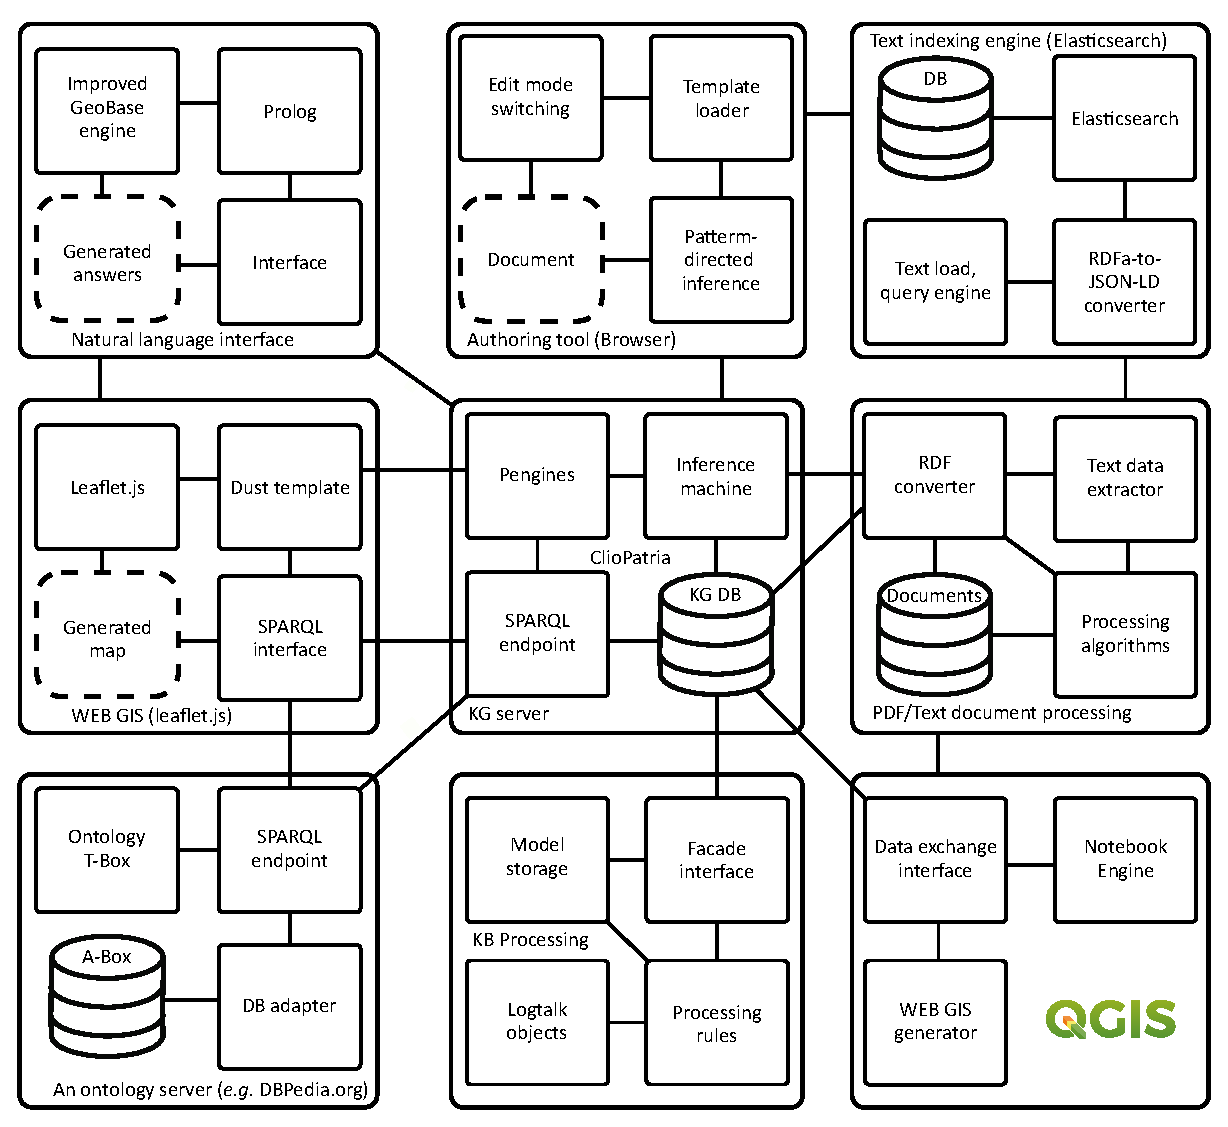
\includegraphics[width=0.8\linewidth]{architecture.pdf}
  \caption{Target architecture of the environment}
  \label{fig:target}
\end{figure}


\section*{Conclusion}

Viewer in essence interprets partially SPARQL-quarries as maps.

\begin{acknowledgments}

\end{acknowledgments}

%%
%% Define the bibliography file to be used
% \bibliography{sample-ceur}

\begin{thebibliography}{99}

\bibitem{hogan} Aidan Hogan, Eva Blomqvist, Michael Cochez, Claudia D’Amato \emph{et al}. Knowledge Graphs. \url{https://arxiv.org/abs/2003.02320v5}
\bibitem{lgd} Claus Stadler, Jens Lehmann, Konrad Höffner, Sören Auer. LinkedGeoData: A core for a web of spatial open data. Semantic Web 3 (2012) 333–354. \doi{10.3233/SW-2011-0052}

\bibitem{iwaniak1} Adam Iwaniak, Iwona Kaczmarek, Marek Strzelecki, Jaromar Lukowicz, Piotr Jankowski. Enriching and improving the quality of linked data with GIS. \doi{10.1515/geo-2016-0c020}

\bibitem{iwaniak17} Adam Iwaniak, Marta Leszczuk, Marek Strzelecki, Francis Harvey, Iwona Kaczmarek. A Novel Approach for Publishing Linked Open Geodata from National Registries with the Use of Semantically Annotated Context Dependent Web Pages. International Journal of Geo-Information. 6, 252, 2017. \doi{10.3390/ijgi6080252}

\bibitem{abid} Tarek Abid, Hafed Zarzour. Integrating Linked Open Data in Geographical
Information System. International Conference on Information Technology for Organization Development. 2014.

\bibitem{geolink} Michelle Cheatham, Adila Krisnadhi, Reihaneh Amini, Pascal Hitzler, \emph{et al} (2018) The GeoLink knowledge graph, Big Earth Data, 2:2, 131-143, \doi{10.1080/20964471.2018.1469291}

\bibitem{lunina} Oksana V. Lunina.  The digital map of the pliocene quaternary crustal faults in the southern east siberia and the adjacent northern Mongolia. Geodynamics \& Tectonophysics. 2016. 7(3):407-434. \doi{10.5800/GT-2016-7-3-0215}
\bibitem{afs} Cartographic service Activetectonics. \url{http://activetectonics.ru/} (access date: 20-Sep-2021)
\bibitem{foss} Mathias Leidig, Richard Teeuw. Free software: A review, in the context of disaster management. 2015. International Journal of Applied Earth Observation and Geoinformation,
Vol.~42, pp.~49-56, ISSN 0303-2434, \doi{10.1016/j.jag.2015.05.012}.

\bibitem{graphdb} 1
\bibitem{protege} 2
\bibitem{python} 3
\bibitem{cliopatria} 3
\bibitem{cherkashin19} d

\bibitem{zont19}  Cherkashin E, Shigarov A and Paramonov V 2019 Representation of MDA transformation with logical objects \emph{International Multi-Conference on Engineering, Computer and Information Sciences (SIBIRCON), Novosibirsk, Russia} 0913--8 \doi{10.1109/SIBIRCON48586.2019.8958008}


\end{thebibliography}

%%
%% If your work has an appendix, this is the place to put it.
\appendix

\section{Online Resources}

The sources for the viewer are being developed at
\href{https://github.com/De17eon/GRL}{GitHub}.

\end{document}

%%
%% End of file

%%% Local Variables:
%%% mode: latex
%%% TeX-master: t
%%% End:
